\def \kaflanr {16}
\lecture[\kaflanr]{\kaflanr. Hagnýtingar margfaldra heilda}{lecture-text}
\date{25.~febrúar 2015}
\newcounter{mycount}
\refstepcounter{mycount}

\begin{document}

\subsection{}
\maketitle





\subsection{Kúluhnit} 

\subsubsection{Skilgreining \kaflanr.\arabic{mycount}}\stepcounter{mycount}
 Látum $(x,y,z)$ vera punkt í $\R^3$.  {\em Kúluhnit} $(x,y,z)$ eru þrennd talna $\rho, \phi, \theta$ þannig að 
$$x=\rho\sin\phi\cos\theta\qquad\qquad y=\rho\sin\phi\sin\theta\qquad\qquad z=\rho\cos\phi.$$
Punktur sem hefur kúluhnit $\rho, \phi, \theta$ er táknaður 
með $[\rho, \phi, \theta]$. 

\begin {figure}[h!]
 \centering
            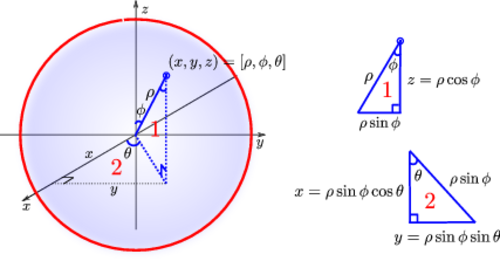
\includegraphics[width=0.75\linewidth]{sphere}
            \caption*{}
\end {figure}




\subsection{} 

\subsubsection{Umræða \kaflanr.\arabic{mycount}}\stepcounter{mycount}
Eftirfarandi jöfnur gefa aðferð til að finna kúluhnit:
\begin{itemize}
\item[$\rho$]  er fjarlægðin frá $(0,0,0)$ til $(x,y,z)$, það er að segja 
$$\rho=\sqrt{x^2+y^2+z^2}.$$
\item[$\phi$] er hornið á milli jákvæða hluta $z$-ássins og línustriksins frá $(0,0,0)$ til $(x,y,z)$.  Hornið $\phi$ má ákvarða út frá jöfnunni
$$\tan\phi=\frac{\sqrt{x^2+y^2}}{z}.$$
\item[$\theta$] er hornið sem jákvæði hluti $x$-ásins myndar við línustrikið frá $(0,0,0)$ til $(x,y,0)$ (sama horn og notað í sívalningshnitum (og pólhnitum)).   Hornið $\theta$ má finna út frá jöfnunni
$$\tan\theta=\frac{y}{x}.$$
\end{itemize}
Um kúluhnit $[\rho, \phi, \theta]$ fyrir punkt $(x,y,z)$ gildir að 
velja má $\rho, \phi, \theta$ þannig að
$0\leq \rho$, $0\leq\phi\leq \pi$ og $0\leq\theta\leq 2\pi$.





\subsection{Breytuskipti í kúluhnit} 

\subsubsection{Setning \kaflanr.\arabic{mycount}}\stepcounter{mycount}
 Látum $R$ vera rúmskika þannig að þegar notuð eru kúluhnit þá fæst eftirfarandi lýsing
$$R=\{[\rho,\phi,\theta]\mid \alpha\leq\theta\leq\beta, 
c\leq\phi\leq d, a\leq \rho\leq b\}.$$ 
Ef $f$ er fall sem er heildanlegt yfir $R$ þá er
\begin{align*}&\thrint_R f(x,y,z)\,dV=\\ &\int_\alpha^\beta\!\int_c^d\!\int_a^b f(\rho\sin\phi\cos\theta, \rho\sin\phi\sin\theta,\rho\cos\phi)
\,\rho^2\sin\phi\,d\rho\,d\phi\,d\theta.
\end{align*}





\subsection{Massamiðja} 

\subsubsection{Regla \kaflanr.\arabic{mycount}}\stepcounter{mycount}
 Látum $D$ tákna svæði í plani.  Hugsum $D$ sem plötu þ.a.~í punkti $(x,y)$ er efnisþéttleikinn gefinn með falli $\delta(x,y)$.  Massi plötunnar er 
$$m=\tvint_D \delta(x,y)\,dA.$$
 {\em Vægi} plötunnar um línuna $x=0$ (þ.e.~$y$-ás) og um línuna $y=0$ (þ.e.~$x$-ás) eru gefin með
 $$M_{x=0}=\tvint_D x\delta(x,y)\,dA \quad \text{og} \quad M_{y=0}=\tvint_D y\delta(x,y)\,dA.$$
Hnit {\em massamiðju} plötunnar eru $(\overline{x}, \overline{y})$ þar sem 
$$\overline{x}=\frac{M_{x=0}}{m}
 \quad \text{og}\quad \overline{y}=\frac{M_{y=0}}{m}.$$






\subsection{} 

\subsubsection{Regla \kaflanr.\arabic{mycount}}\stepcounter{mycount}
 Látum $R$ tákna rúmskika.  Hugsum $R$ sem hlut þannig að í punkti $(x,y,z)$ er efnisþéttleikinn gefinn með falli $\delta(x,y,z)$.  Massi hlutarins er 
$$m=\thrint_R \delta(x,y,z)\,dV.$$
 {\em Vægi} hlutarins um planið $x=0$ (þ.e.~$yz$-planið) er
 $$M_{x=0}=\thrint_R x\delta(x,y,z)\,dV.$$
 Svipað skilgreinum við
 $$M_{y=0}=\thrint_R y\delta(x,y,z)\,dV 
 \quad \text{og}\quad
 M_{z=0}=\thrint_R z\delta(x,y,z)\,dV.$$
Hnit {\em massamiðju} hlutarins eru $(\overline{x}, \overline{y}, \overline{z})$ þar sem 
$$\overline{x}=\frac{M_{x=0}}{m}
\qquad\mbox{og}\qquad
\overline{y}=\frac{M_{y=0}}{m}
\qquad\mbox{og}\qquad
\overline{z}=\frac{M_{z=0}}{m}.$$





\subsection{Hverfitregða} 

\subsubsection{Regla \kaflanr.\arabic{mycount}}\stepcounter{mycount}
 Látum $R$ tákna rúmskika.  Hugsum $R$ sem hlut þannig að í punkti $(x,y,z)$ er efnisþéttleikinn gefinn með falli $\delta(x,y,z)$.  Látum $L$ tákna línu (snúningsás) í rúminu. {\em Hverfitregða} hlutarins um $L$ er
$$I=\thrint_R D^2 \,\delta\,dV$$
þar sem $\delta=\delta(x,y,z)$ og $D=D(x,y,z)$ er fjarlægð punktsins $(x,y,z)$ frá $L$.





\subsection{Yfirborðsflatarmál} 

\subsubsection{Regla \kaflanr.\arabic{mycount}}\stepcounter{mycount}
 Látum $D$ vera svæði í plani og $f(x,y)$ diffranlegt fall skilgreint á $D$.  Flatarmál grafsins $z=f(x,y)$ þar sem $(x,y)\in D$ er gefið með formúlunni
$$S=\tvint_D \sqrt{1+f_1(x,y)^2+f_2(x,y)^2}\,dA.$$






\end{document}